\documentclass[11pt]{article}

\usepackage{amsmath,amssymb}
\usepackage{amsthm}
\usepackage{graphicx}
\usepackage{booktabs}
\usepackage{hyperref}
\usepackage{geometry}
\usepackage{algorithm}
\usepackage{algpseudocode}
\usepackage{caption}
\usepackage{subcaption}
\usepackage{tikz}
\usepackage{pgfplots}
\usepackage{placeins}
\usepackage{float}
\pgfplotsset{compat=1.18}
\usetikzlibrary{positioning,arrows.meta,patterns,calc,decorations.pathreplacing,pgfplots.fillbetween}

\geometry{margin=1in}

% Theorem environments
\newtheorem{theorem}{Theorem}
\newtheorem{lemma}[theorem]{Lemma}
\newtheorem{corollary}[theorem]{Corollary}
\newtheorem{proposition}[theorem]{Proposition}
\theoremstyle{definition}
\newtheorem{definition}[theorem]{Definition}
\newtheorem{example}[theorem]{Example}
\theoremstyle{remark}
\newtheorem{remark}[theorem]{Remark}
\newtheorem{claim}[theorem]{Claim}

\title{DeltaSort: Incremental repair of sorted arrays with known updates}
\author{Shubham Dwivedi \\
\small Independent Researcher \\
\small \texttt{shubd3@gmail.com}
}
\date{January 2026}

\begin{document}
\maketitle

\begin{abstract}
Maintaining sorted order under incremental updates is a common requirement in read-heavy systems,
yet most production sorting routines are blind to which elements have changed and must repeatedly
rediscover partial order from scratch. This paper explores an alternative model in which the sorting
routine is explicitly informed of the indices updated since the previous sort. Under this model,
we present \emph{DeltaSort}, an incremental repair algorithm for arrays that batches multiple
updates instead of applying them independently. \emph{DeltaSort} reduces redundant comparison work
and overlapping data movement by exploiting update locality and batching. An experimental evaluation
of a Rust implementation shows that \emph{DeltaSort} outperforms repeated Binary-Insertion-Sort
and NativeSort for update batch sizes up to ~25\%, with multi-fold speedups and a clear
crossover point depending on array size where full re-sorting becomes preferable. These results
suggest that tighter integration between update pipelines and sorting routines can yield significant
performance gains in real incremental-sorting workloads at the cost of increased memory usage to
track updated indices.
\end{abstract}

%==============================================================================
\section{Introduction}
%==============================================================================

Sorting is among the most heavily optimized primitives in modern systems. Standard library
implementations—TimSort~\cite{timsort}, Introsort~\cite{musser1997introspective}, and
PDQSort~\cite{peters2021pdqsort}—deliver excellent performance for general inputs by
exploiting partial order, cache locality, and adaptive strategies. However, these algorithms
operate under a \emph{blind} model: they rediscover structure dynamically rather than being
explicitly informed about which elements have changed since the previous sort.

In many practical systems, this assumption is unnecessarily pessimistic. Sorted arrays are
often maintained incrementally in read-heavy workloads where updates affect only a subset
of elements and the indices of those updates can be easily tracked and known. Nevertheless,
this information is typically not tracked or utilized, and systems fall back to blind re-sorting
or independent incremental repairs using binary-insertion or extract-sort-merge. To address
these limitations, this paper makes the following contributions:

\begin{enumerate}
  \item \textbf{Update-aware sorting model:}
  We formulate an incremental sorting model in which the sorting routine is explicitly
  informed of the indices updated since the previous sort. Under this model, a natural
  baseline is repeated binary insertion, where each update is repaired independently using
  binary search. While correct, this approach exhibits efficiency limitations for batched
  updates due to repeated full-range searches and overlapping data movement.

  \item \textbf{DeltaSort algorithm:}
  We present \emph{DeltaSort}, an incremental repair algorithm for sorted arrays
  designed for the update-aware model. DeltaSort batches updates and repairs them jointly,
  reducing redundant comparison work and overlapping element movement by exploiting update
  locality and batching. DeltaSort preserves correctness and does not improve asymptotic
  complexity, but achieves consistent practical performance improvements over repeated
  binary insertion and blind native sorting in relevant update regimes.
\end{enumerate}

%==============================================================================
\section{Related Work}
\label{sec:related}
%==============================================================================

Adaptive sorting algorithms exploit existing order in the input to improve performance on
nearly sorted data. TimSort~\cite{timsort} and natural merge sort~\cite{knuth1998art} identify
monotonic runs dynamically and merge them efficiently, yielding improved performance when
such structure is present. A substantial body of work formalizes measures of presortedness
and studies sorting algorithms whose complexity depends on these measures rather than input
size alone~\cite{mannila1985measures}. These approaches, however, must discover structure
through full-array scans and do not assume explicit knowledge of which elements were modified.

Dynamic data structures offer a different trade-off. Self-balancing trees such as AVL
trees~\cite{avl1962}, red--black trees~\cite{guibas1978dichromatic}, B-trees~\cite{bayer1970organization},
and skip lists~\cite{pugh1990skip} support efficient ordered updates with logarithmic cost,
but sacrifice contiguous memory layout and cache locality. Library sort~\cite{bender2006insertion}
reduces insertion cost by maintaining gaps in the array, but addresses online insertion and
incurs additional space overhead.

In contrast, this work focuses on maintaining sorted order in arrays under batched updates
where the indices of modified elements are explicitly available. This update-aware model
enables efficient repair without auxiliary data structures or additional memory, and
distinguishes DeltaSort from prior adaptive and incremental approaches.

%==============================================================================
\section{Problem Model}
\label{sec:model}
%==============================================================================

\begin{definition}[Update-Aware Sorting]
\label{def:problem}
Let $A[0..n-1]$ be an array sorted according to a strict weak ordering
defined by a comparator $\texttt{cmp}$. Suppose a set of indices
$D = \{d_1, \ldots, d_k\} \subseteq \{0, \ldots, n-1\}$ is given such that
the values at these indices may have been arbitrarily modified, while
values at all other indices remain unchanged.

The \emph{update-aware sorting problem} is to restore $A$ to a state that
is sorted with respect to $\texttt{cmp}$, given explicit knowledge of the
set $D$.
\end{definition}

%==============================================================================
\section{DeltaSort Algorithm}
\label{sec:algorithm}
%==============================================================================

\subsection{Overview}

\begin{definition}[Violation]
\label{def:violation}
For a dirty index $i$, we classify its \emph{violation} based on local order:
\begin{itemize}
  \item \textbf{LEFT (L)}: Element \textbf{must} move left — $\texttt{cmp}(A[i-1], A[i]) > 0$ (for $i > 0$).
  \item \textbf{RIGHT (R)}: Element \textbf{may} move right or stay stable. Essentially, all dirty indices that are not LEFT.
\end{itemize}
\end{definition}

\begin{definition}[Segment]
\label{def:segment}
A \emph{segment} is a maximal group of dirty indices with structure
$(\textrm{R})^*\textrm{L}^+$: zero or more RIGHT dirty indices
followed by one or more LEFT dirty indices. Clean elements may be interspersed
between dirty indices within a segment.

\end{definition}

% Figure: Segment structure diagram
\begin{figure}[h]
\centering
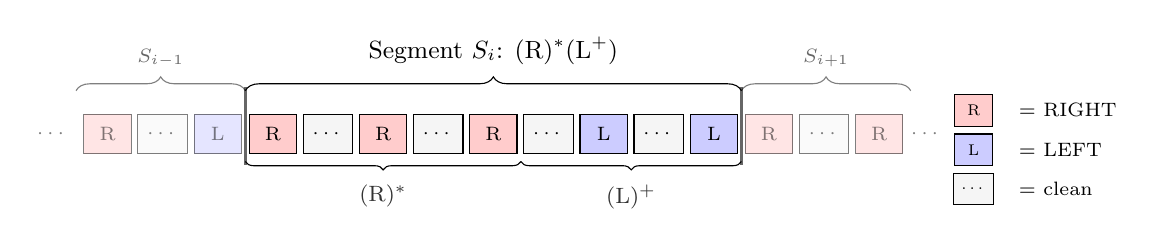
\begin{tikzpicture}[
    cell/.style={minimum width=0.6cm, minimum height=0.5cm, draw, font=\scriptsize},
    dotcell/.style={minimum width=0.5cm, minimum height=0.5cm, font=\scriptsize},
    right/.style={cell, fill=red!20},
    left/.style={cell, fill=blue!20},
    clean/.style={cell, fill=gray!8},
    boundary/.style={very thick, black!60},
    segbrace/.style={decorate, decoration={brace, amplitude=5pt}},
    subbrace/.style={decorate, decoration={brace, amplitude=3pt, mirror}},
    seglabel/.style={font=\footnotesize, text=black!80},
    faded/.style={opacity=0.5}
]

% === PREVIOUS SEGMENT (faded) ===
\begin{scope}[faded]
  \node[dotcell] at (-1.4, 0) {$\cdots$};
  \node[right] (pr1) at (-0.7, 0) {R};
  \node[clean] at (0, 0) {$\cdots$};
  \node[left] (pl1) at (0.7, 0) {L};
\end{scope}

% Boundary: previous segment | current segment
\draw[boundary] (1.05, 0.6) -- (1.05, -0.4);

% === CURRENT SEGMENT (main focus) ===
% RIGHT region: R [...] R [...] R
\node[right] (r1) at (1.4, 0) {R};
\node[clean] at (2.1, 0) {$\cdots$};
\node[right] (r2) at (2.8, 0) {R};
\node[clean] at (3.5, 0) {$\cdots$};
\node[right] (r3) at (4.2, 0) {R};

% LEFT region: [...] L [...] L
\node[clean] at (4.9, 0) {$\cdots$};
\node[left] (l1) at (5.6, 0) {L};
\node[clean] at (6.3, 0) {$\cdots$};
\node[left] (l2) at (7.0, 0) {L};

% Boundary: current segment | next segment
\draw[boundary] (7.35, 0.6) -- (7.35, -0.4);

% === NEXT SEGMENT (faded) ===
\begin{scope}[faded]
  \node[right] (nr1) at (7.7, 0) {R};
  \node[clean] at (8.4, 0) {$\cdots$};
  \node[right] (nr2) at (9.1, 0) {R};
  \node[dotcell] at (9.7, 0) {$\cdots$};
\end{scope}

% === ANNOTATIONS ===
% Main segment brace (top)
\draw[segbrace] (1.05, 0.55) -- (7.35, 0.55) 
    node[midway, above=6pt, font=\small] {Segment $S_i$: $(\mathrm{R})^*(\mathrm{L}^+)$};

% Sub-braces (bottom)
\draw[subbrace] (1.05, -0.35) -- (4.55, -0.35) 
    node[midway, below=5pt, seglabel, align=center] {$(\mathrm{R})^*$};
\draw[subbrace] (4.55, -0.35) -- (7.35, -0.35) 
    node[midway, below=5pt, seglabel, align=center] {$(\mathrm{L})^+$};

% Adjacent segment labels (above, smaller)
\draw[segbrace, faded] (-1.1, 0.55) -- (1.05, 0.55) 
    node[midway, above=5pt, font=\scriptsize, opacity=0.6] {$S_{i-1}$};
\draw[segbrace, faded] (7.35, 0.55) -- (9.5, 0.55) 
    node[midway, above=5pt, font=\scriptsize, opacity=0.6] {$S_{i+1}$};

% Legend
\node[right, scale=0.8] at (10.3, 0.3) {R};
\node[font=\scriptsize, anchor=west] at (10.75, 0.3) {= RIGHT};
\node[left, scale=0.8] at (10.3, -0.2) {L};
\node[font=\scriptsize, anchor=west] at (10.75, -0.2) {= LEFT};
\node[clean, scale=0.8] at (10.3, -0.7) {$\cdots$};
\node[font=\scriptsize, anchor=west] at (10.75, -0.7) {= clean};

\end{tikzpicture}
\caption{Segment structure after Phase~1. Each segment follows the pattern $(\mathrm{R})^*(\mathrm{L}^+ \mid \epsilon)$: zero or more RIGHT violations followed by one or more LEFT violations.}
\label{fig:segment-diagram}
\end{figure}


DeltaSort operates in two phases:

\begin{enumerate}
  \item \textbf{Phase 1 (Preparation):} Extract dirty values, sort them, write back to
        dirty positions in index order. This establishes direction segments in the array which
        are disjoint and can be repaired independently.
  \item \textbf{Phase 2 (Repair):} Repair each segment left-to-right, deferring RIGHT indices
        to a stack until the first LEFT index is encountered. Flush and repair the the RIGHT
        indexes in stack in LIFO order. Then repair all LEFT indices left-to-right.
\end{enumerate}

\subsection{Key Insight: Directional segmentation enables localized repair}
\label{sec:insight}

The key insight behind DeltaSort is that pre-sorting dirty values induces a
\emph{directional segmentation} of updates. After Phase~1, dirty indices partition
into disjoint segments of the form $(\textrm{R})^*\textrm{L}^+$.

\begin{lemma}[Movement Confinement]
\label{lem:confinement}
Element movement is bounded within each segment: no element crosses a segment boundary.
\end{lemma}

\begin{proof}
Let $S$ be a segment with RIGHT indices $R_1, \ldots, R_m$ followed by LEFT indices
$L_1, \ldots, L_p$. After Phase~1, dirty values are monotonically ordered by index,
so $A[R_1] < \cdots < A[R_m] < A[L_1] < \cdots < A[L_p]$.

\begin{enumerate}
  \item \emph{RIGHT elements cannot pass the leftmost LEFT.}
        Since $A[R_i] < A[L_1]$ for all $i$.

  \item \emph{LEFT elements cannot pass the rightmost RIGHT.}
        Since $A[R_m] < A[L_j]$ for all $j$.
\end{enumerate}

Since no element exits its segment, segments can be repaired independently.
\end{proof}

\subsection{Detailed Algorithm}

\begin{algorithm}[H]
\caption{DeltaSort}
\label{alg:deltasort}
\begin{algorithmic}[1]
\Require Array $A[0..n-1]$, dirty indices $D$, comparator $\texttt{cmp}$
\Ensure $A$ is sorted
\Statex
\State \textbf{Phase 1: Prepare}
\State $\texttt{dirty} \gets \text{sort}(D)$ \Comment{Sort indices ascending}
\State $\texttt{values} \gets [A[d] : d \in \texttt{dirty}]$
\State $\texttt{values} \gets \text{sort}(\texttt{values}, \texttt{cmp})$
\For{$i \gets 0$ \textbf{to} $|\texttt{dirty}| - 1$}
    \State $A[\texttt{dirty}[i]] \gets \texttt{values}[i]$
\EndFor
\Statex
\State \textbf{Phase 2: Repair}
\State $\texttt{pending} \gets []$; $\texttt{leftBound} \gets 0$
\For{$p \gets 0$ \textbf{to} $|\texttt{dirty}| - 1$}
    \State $i \gets \texttt{dirty}[p]$
    \If{$\Call{IsLeftViolation}{A, i}$}
        \State \Call{FlushPending}{$\texttt{pending}, i-1$} \Comment{Fix pending before LEFT}
        \State $\texttt{leftBound} \gets \Call{FixLeftViolation}{A, i, \texttt{leftBound}} + 1$
    \Else
        \State $\texttt{pending.push}(i)$ \Comment{Defer RIGHT indices}
    \EndIf
\EndFor
\Statex
\State \Call{FlushPending}{$\texttt{pending}, n-1$} \Comment{Fix remaining RIGHT violations}
\end{algorithmic}
\end{algorithm}

\vspace{0.5em}

\noindent\begin{minipage}{\linewidth}
\begin{algorithmic}[1]
\Function{IsLeftViolation}{$A$, $i$}
    \State \Return $i > 0 \land \texttt{cmp}(A[i-1], A[i]) > 0$
\EndFunction
\Statex
\Function{IsRightViolation}{$A$, $i$}
    \State \Return $i < n-1 \land \texttt{cmp}(A[i], A[i+1]) > 0$
\EndFunction
\end{algorithmic}
\end{minipage}

\vspace{0.5em}

\noindent\begin{minipage}{\linewidth}
\begin{algorithmic}[1]
\Function{FixLeftViolation}{$A$, $i$, $\texttt{leftBound}$}
    \State $t \gets \Call{BinarySearchLeft}{A, A[i], \texttt{leftBound}, i-1}$
    \State \Call{Move}{A, i, t}
    \State \Return $t$
\EndFunction
\end{algorithmic}
\end{minipage}

\vspace{0.5em}

\noindent\begin{minipage}{\linewidth}
\begin{algorithmic}[1]
\Function{FlushPending}{$\texttt{pending}$, $\texttt{rightBound}$}
    \While{$\texttt{pending} \neq \emptyset$}
        \State $s \gets \texttt{pending.pop}()$ \Comment{Process in LIFO order}
        \If{$\Call{IsRightViolation}{A, s}$}
            \State $t \gets \Call{BinarySearchRight}{A, A[s], s+1, \texttt{rightBound}}$
            \State \Call{Move}{A, s, t}
        \EndIf
    \EndWhile
\EndFunction
\end{algorithmic}
\end{minipage}

\vspace{0.5em}

\noindent\begin{minipage}{\linewidth}
\begin{algorithmic}[1]
\Function{Move}{$A$, $from$, $to$}
    \State $v \gets A[from]$
    \If{$from < to$}
        \State Shift $A[from+1..to]$ left by one
    \ElsIf{$from > to$}
        \State Shift $A[to..from-1]$ right by one
    \EndIf
    \State $A[to] \gets v$
\EndFunction
\end{algorithmic}
\end{minipage}


\subsection{Correctness Proof}

\begin{claim}[Segment Boundary Invariant]
\label{claim:boundary-invariant}
Segment boundaries are never violated. For any two consecutive segments $S_i$ and 
$S_{i+1}$, all values in $S_i$ remain less than all values in $S_{i+1}$ throughout 
the repair process.
\end{claim}

\begin{proof}[Proof sketch]
After Phase~1, dirty values are monotonically ordered by index. A segment boundary 
occurs where a LEFT dirty index is followed by a RIGHT dirty index. At such a 
boundary, the RIGHT element satisfies $A[d_{i+1}] \geq A[d_{i+1}-1]$, establishing 
sorted order. By Lemma~\ref{lem:confinement}, movement is confined within segments, 
so boundaries remain intact. A fully rigorous proof is deferred to future work.
\end{proof}

\begin{lemma}[Fixing Does Not Introduce Violations]
\label{lem:fix-invariant}
When a LEFT or RIGHT element is moved to its correct position via binary search, 
no new violations are introduced.
\end{lemma}

\begin{proof}
\emph{LEFT fix}: Binary search finds position $t < i$ where the element belongs. 
Elements in $A[t..i-1]$ shift right by one. The shift preserves relative order. 
By binary search, the moved element satisfies $A[t-1] \leq A[t] < A[t+1]$.

\emph{RIGHT fix}: Binary search finds position $t > s$ where the element belongs. 
Elements in $A[s+1..t]$ shift left by one. The shift preserves relative order. 
By binary search, the moved element satisfies $A[t-1] < A[t] \leq A[t+1]$.

In both cases, no new violations are introduced.
\end{proof}

\begin{theorem}[Correctness]
\label{thm:correctness}
DeltaSort produces a correctly sorted array.
\end{theorem}

\begin{proof}
Phase~2 processes each dirty index exactly once, fixing its violation if any. 
By Lemma~\ref{lem:fix-invariant}, each fix resolves a violation without 
introducing new ones. After all dirty indices are processed, each segment 
is internally sorted.

By Claim~\ref{claim:boundary-invariant}, segment boundaries maintain sorted 
order throughout. Since each segment is internally sorted and boundaries 
preserve global order, the entire array is sorted.
\end{proof}

\subsection{Algorithm Analysis}

\begin{theorem}[Time Complexity]
\label{thm:time}
DeltaSort runs in $O(k \log k + k \log n + M)$ time, where $M$ is total movement.
\end{theorem}

\begin{proof}
\textbf{Phase 1}: Sort $k$ indices: $O(k \log k)$. Sort $k$ values: $O(k \log k)$.
Write back: $O(k)$.

\textbf{Phase 2}: Each dirty index: $O(1)$ direction check, $O(\log n)$ binary search.
Total: $O(k \log n)$. Movement: $O(M)$.
\end{proof}

\begin{theorem}[Space Complexity]
\label{thm:space}
DeltaSort uses $O(k)$ auxiliary space.
\end{theorem}

\begin{remark}[Movement Efficiency]
While worst-case movement is $O(kn)$, the segmentation created by Phase 1 tends to
reduce movement in practice in the average case. Empirical results in \S\ref{sec:experiments}
demonstrate substantial speedups, validating that movement is typically much less than the worst case.
\end{remark}

Here we compare algorithm complexity with other standard baseline approaches which we use in experiments
to compare DeltaSort's performance:
\begin{itemize}
  \item \textbf{NativeSort (NS)}: Re-sort the array using the natively available sort function.
  $O(n \log n)$ comparisons and movements.
  \item \textbf{Binary-Insertion-Sort (BIS)}: Extract dirty values, then for each: 
        binary search for correct position, reinsert. $O(k \log n)$ comparisons, 
        $O(kn)$ worst-case movement. Searches the full array range for each insertion.
  \item \textbf{Extract-Sort-Merge (ESM)}: Extract dirty values, sort them, merge 
        with clean elements. $O(k \log k + n)$ comparisons, $O(n)$ movement. 
        Requires $O(n)$ auxiliary space.
\end{itemize}

\begin{table}[h]
\centering
\caption{Algorithm complexity comparison.}
\label{tab:complexity}
\begin{tabular}{l c c c c}
\toprule
Algorithm & Comparisons & Movement & Space \\
\midrule
NativeSort & $O(n \log n)$ & $O(n \log n)$ & $O(n)$ \\
Binary-Insertion-Sort & $O(k \log n)$ & $O(kn)$ & $O(1)$ \\
Extract-Sort-Merge & $O(k \log k + n)$ & $O(n)$ & $O(n)$ \\
\textbf{DeltaSort} & $O(k \log n)$ & $O(kn)$* & $O(k)$ \\
\bottomrule
\end{tabular}

\vspace{0.3em}
{\small *Worst case; average case is closer to $O(n)$.}
\end{table}

%==============================================================================
\section{Experimental Evaluation}
\label{sec:experiments}
%==============================================================================

All experiments are run using a Rust implementation of DeltaSort~\cite{deltasort-repo} on a synthetic dataset
of user objects with composite keys (country, age, name) on a M3 Pro Macbook Pro with 18GB RAM. DeltaSort is compared against
three baselines: Native sort (Rust's \texttt{sort\_by}), Binary Insertion Sort (BIS),
and Extract-Sort-Merge (ESM).

\subsection{Correctness}
Correctness is verified by an extensive set of randomized unit tests~\cite{deltasort-repo} across various scales and
update sizes. The test routine generates a sorted base array of size $N$, applies $k$ random
updates at random indices, runs DeltaSort, and asserts that the final array is sorted and contains
all original elements with updated values. All tests pass successfully.

\subsection{Execution Time}

The graph below shows execution time (in microseconds) for $n = 50,000$ elements
as a function of dirty count $k$. DeltaSort consistently outperforms all alternatives
up to approximately $k = 15K$ (crossover point), achieving significant speedups of 6--20$\times$
over Native sort in the intermediate range. Also note the orders-of-magnitude gap between
DeltaSort and the baseline incremental algorithms (BIS and ESM) across the full range of
$k$ values.

% Figure: All algorithms comparison (log-log scale)
\begin{figure}[H]
\centering
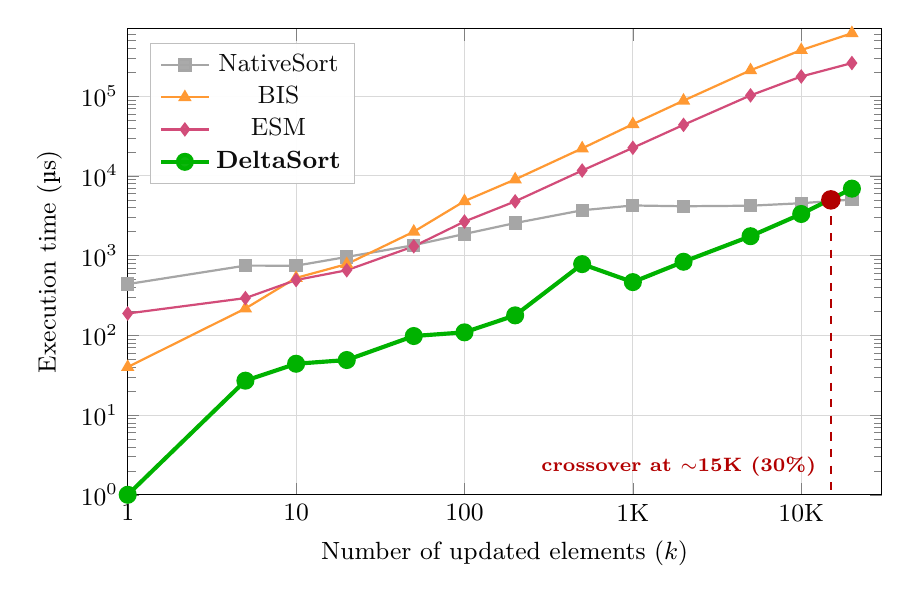
\begin{tikzpicture}
\begin{axis}[
    width=0.92\textwidth,
    height=7.5cm,
    xlabel={Number of updated elements ($k$)},
    ylabel={Execution time (\textmu s)},
    xmode=log,
    ymode=log,
    log basis x=10,
    log basis y=10,
    xmin=1, xmax=30000,
    ymin=1, ymax=700000,
    xtick={1, 10, 100, 1000, 10000},
    xticklabels={1, 10, 100, 1K, 10K},
    legend pos=north west,
    legend style={font=\small, fill=white, fill opacity=0.95, draw=gray!50},
    grid=major,
    major grid style={line width=0.3pt, draw=gray!30},
    tick label style={font=\small},
    label style={font=\small},
]

% NativeSort (horizontal-ish baseline)
\addplot[color=gray!70, mark=square*, thick, mark size=2pt] coordinates {
    (1, 439) (5, 749) (10, 747) (20, 962) (50, 1350) (100, 1867) 
    (200, 2560) (500, 3703) (1000, 4253) (2000, 4158) 
    (5000, 4223) (10000, 4539) (20000, 5042)
};

% Binary Insertion (steep slope)
\addplot[color=orange!80, mark=triangle*, thick, mark size=2pt] coordinates {
    (1, 40) (5, 217) (10, 525) (20, 782) (50, 1994) (100, 4818) 
    (200, 9022) (500, 22112) (1000, 44481) (2000, 87827) 
    (5000, 211016) (10000, 377981) (20000, 615645)
};

% Extract-Sort-Merge
\addplot[color=purple!70, mark=diamond*, thick, mark size=2pt] coordinates {
    (1, 188) (5, 293) (10, 494) (20, 655) (50, 1307) (100, 2673) 
    (200, 4785) (500, 11655) (1000, 22480) (2000, 43627) 
    (5000, 102198) (10000, 176373) (20000, 259835)
};

% DeltaSort (our algorithm - emphasized)
\addplot[color=green!70!black, mark=*, thick, mark size=2.5pt, line width=1.5pt] coordinates {
    (1, 1) (5, 27) (10, 44) (20, 49) (50, 98) (100, 109) 
    (200, 178) (500, 782) (1000, 465) (2000, 837) 
    (5000, 1751) (10000, 3326) (20000, 6914)
};

% Crossover point: bold marker + dashed drop line + label
\node[circle, fill=red!70!black, inner sep=2.5pt] at (axis cs:15000, 5000) {};
\draw[red!70!black, thick, dashed] (axis cs:15000, 5000) -- (axis cs:15000, 1);
\node[font=\scriptsize\bfseries, text=red!70!black, anchor=north east] at (axis cs:14000, 4) {crossover at $\sim$15K (30\%)};

\legend{NativeSort, BIS, ESM, \textbf{DeltaSort}}
\end{axis}
\end{tikzpicture}
\caption{Execution time comparison for $n = 50{,}000$ elements (log-log scale). The vertical dashed line marks the crossover point ($k \approx 15$K) where DeltaSort's advantage over NativeSort diminishes. The shaded region indicates where DeltaSort outperforms all alternatives.}
\label{fig:all-algorithms}
\end{figure}


\subsection{Comparator Invocation Count}

The following chart shows the number of comparator invocations for each algorithm. DeltaSort
and Binary Insertion both achieve $O(k \log n)$ comparisons, substantially fewer than Native
sort's $O(n \log n)$ and ESM's $O(k \log k + n)$. The comparison counts for DeltaSort are 10-40\%
more than BI , confirming that DeltaSort's performance advantage comes from reduced data movement.

% Figure: Comparator invocation count comparison
\begin{figure}[H]
\centering
\begin{tikzpicture}
\begin{axis}[
    width=0.92\textwidth,
    height=6cm,
    xlabel={Number of updated values ($k$)},
    ylabel={Comparator invocations},
    xmode=log,
    ymode=log,
    log basis x=10,
    log basis y=10,
    xmin=1, xmax=100000,
    ymin=10, ymax=10000000,
    xtick={1, 10, 100, 1000, 10000},
    xticklabels={1, 10, 100, 1K, 10K},
    ytick={10, 100, 1000, 10000, 100000, 1000000, 10000000},
    yticklabels={10, 100, 1K, 10K, 100K, 1M, 10M},
    legend pos=south east,
    legend style={font=\small},
    grid=both,
    grid style={line width=0.1pt, draw=gray!30},
    major grid style={line width=0.2pt, draw=gray!50},
]

% Native Sort
\addplot[color=gray!70, mark=square*, thick, mark size=2.5pt] 
    table[col sep=comma, x=k, y=native] {\rootdir/figures/rust/comparator-count.csv};

% Binary Insertion
\addplot[color=orange!80, mark=triangle*, thick, mark size=2.5pt] 
    table[col sep=comma, x=k, y=bis] {\rootdir/figures/rust/comparator-count.csv};

% Extract-Sort-Merge
\addplot[color=purple!70, mark=diamond*, thick, mark size=2.5pt] 
    table[col sep=comma, x=k, y=esm] {\rootdir/figures/rust/comparator-count.csv};

% DeltaSort (emphasized)
\addplot[color=green!70!black, mark=*, thick, mark size=2.5pt, line width=1.5pt] 
    table[col sep=comma, x=k, y=deltasort] {\rootdir/figures/rust/comparator-count.csv};

\legend{NativeSort, BIS, ESM, \textbf{DeltaSort}}
\end{axis}
\end{tikzpicture}
\caption{Comparator invocation count for $n = 50$K. DeltaSort and BIS
both achieve $O(k \log n)$ comparisons, while NativeSort uses $O(n \log n)$ regardless
of $k$, and ESM uses $O(k \log k + n)$. The 10--40\% higher comparison counts for DeltaSort
vs BIS confirm that movement confinement (Lemma~\ref{lem:confinement}) is the major factor in DeltaSort speedup.\rustbenchmarknote}
\label{fig:rust-comparator-count}
\end{figure}


\subsection{Crossover Threshold Analysis}

A key practical question is: at what delta size should one switch from DeltaSort to
Native sort? A binary search was conducted for the crossover point $k_c$ across array
sizes from 1K to 10M elements.

Figure~\ref{fig:crossover-ratio} visualizes how the crossover ratio $k_c / n$ varies 
with array size. The ratio peaks around 31\% for medium-sized arrays ($n \approx 50$K) 
and declines for very large arrays, suggesting that DeltaSort's advantage 
narrows arrays grow very large. More study is needed to understand this trend fully.

% Figure: Crossover ratio vs array size
\begin{figure}[H]
\centering
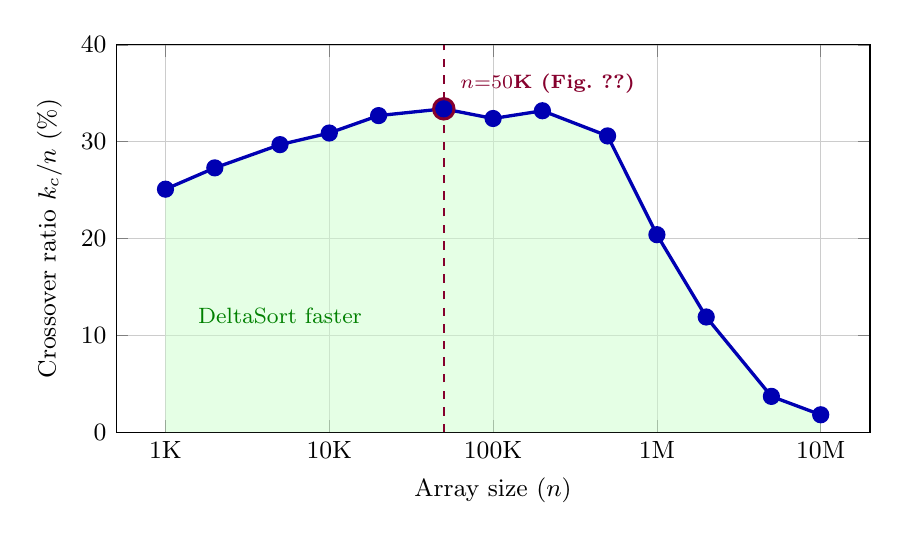
\begin{tikzpicture}
\begin{axis}[
    width=0.92\textwidth,
    height=6.5cm,
    xlabel={Array size ($n$)},
    ylabel={Crossover ratio $k_c / n$ (\%)},
    xmode=log,
    log basis x=10,
    xmin=500, xmax=20000000,
    ymin=0, ymax=40,
    ytick={0, 10, 20, 30, 40},
    yticklabels={0, 10, 20, 30, 40},
    xtick={1000, 10000, 100000, 1000000, 10000000},
    xticklabels={1K, 10K, 100K, 1M, 10M},
    legend pos=north east,
    legend style={font=\small, fill=white, fill opacity=0.95, draw=gray!50},
    grid=both,
    grid style={line width=0.1pt, draw=gray!20},
    major grid style={line width=0.2pt, draw=gray!40},
    tick label style={font=\small},
    label style={font=\small},
]

% Shaded region below the curve (DeltaSort wins)
\addplot[name path=curve, color=blue!70!black, mark=*, thick, mark size=2.5pt, line width=1.2pt] coordinates {
    (1000, 25.1) (2000, 27.3) (5000, 29.7) (10000, 30.9) 
    (20000, 32.7) (50000, 33.4) (100000, 32.4) (200000, 33.2) 
    (500000, 30.6) (1000000, 20.4) (2000000, 11.9) (5000000, 3.7) (10000000, 1.8)
};
\path[name path=bottom] (axis cs:1000,0) -- (axis cs:10000000,0);
\addplot[green!20, opacity=0.5] fill between[of=curve and bottom];

% Vertical line at n=50K (the case evaluated in execution time chart)
\draw[purple!70!black, thick, dashed] (axis cs:50000, 0) -- (axis cs:50000, 40);
\node[circle, fill=purple!70!black, inner sep=3pt] at (axis cs:50000, 33.4) {};
\node[font=\scriptsize\bfseries, text=purple!70!black, anchor=south west] at (axis cs:55000, 34) {$n{=}50$K (Fig.~\ref{fig:all-algorithms})};

% Annotation for the region
\node[font=\footnotesize, text=green!50!black] at (axis cs:5000, 12) {DeltaSort faster};

\end{axis}
\end{tikzpicture}
\caption{Crossover ratio $k_c / n$ as a function of array size. DeltaSort outperforms NativeSort when the updated fraction is below the curve (shaded region).}
\label{fig:crossover-ratio}
\end{figure}


The key takeway is that DeltaSort is beneficial for \textbf{large} ranges of update sizes.
So DeltaSort remains a viable choice even when delta sizes are large. The exact threshold
depends on the scenario specifics (array sizes, data types, comparator cost, etc.) but
the results suggest that a \textbf{25\% dirty fraction} is a reasonable rule of thumb
for the upper limit of delta size before which DeltaSort remains advantageous.

\subsection{Performance in managed execution environments}

DeltaSort was also implemented in JavaScript~\cite{deltasort-repo} running on Node.js v20 (V8 engine). While
the implementation passes all correctness tests, the performance results show higher
variance due to JIT compilation behavior, garbage collection pauses, and other
engine-level effects. The JavaScript benchmarks will be refined in a future revision
to provide more stable measurements. The Rust implementation provides the authoritative
performance characterization.

\section{Future Work}
\label{sec:future}
%==============================================================================

This work suggests several directions for future investigation:

\begin{itemize}
  \item \textbf{Stronger theoretical characterization:}
  While the correctness argument and extensive randomized testing establish that
  DeltaSort produces a correctly sorted array, certain invariants—particularly those governing
  inter-segment boundaries—deserve a more formal treatment that could yield
  sharper theoretical guarantees.

  \item \textbf{Average-case movement bounds:}
  Beyond worst-case correctness and empirical evaluation, establishing
  average-case bounds on data movement under reasonable update distributions
  may help explain observed crossover behavior and clarify when coordinated
  repair is most effective.

  \item \textbf{Structured workload analysis:}
  The current evaluation relies on randomized updates, whereas many real
  workloads exhibit additional structure, such as gradual value changes in
  leaderboards or localized updates in interactive list views. Studying such
  patterns may reveal regimes where DeltaSort’s advantages are amplified or
  diminished.

  \item \textbf{Runtime variance analysis.}
  Performance variance in managed runtimes warrants deeper investigation.
  Understanding the impact of factors such as memory allocation, garbage
  collection, and JIT compilation could improve result interpretability and
  guide implementation choices.

  \item \textbf{Block-structured storage.}
  Although this work focuses on in-memory arrays, the update-aware model
  naturally extends to block-structured storage. Exploring how DeltaSort-style
  coordination interacts with page- or block-based layouts may clarify its
  applicability to database and external-memory settings.
\end{itemize}

%==============================================================================

\section{Conclusion}
\label{sec:conclusion}
%==============================================================================

This paper introduced \emph{DeltaSort}, an incremental repair algorithm for maintaining
sorted arrays under batched updates. The central insight is that pre-sorting updated values
induces \emph{directional segmentation}: dirty elements naturally partition into segments that
can be repaired independently.

DeltaSort leverages this segmentation through stack-based processing. LEFT-moving elements
are repaired immediately with progressively narrowed search ranges, while RIGHT-moving
elements are deferred and processed in reverse order to ensure stable target positions.
This coordination avoids redundant comparisons and overlapping element movement that arise
from repeated binary insertion.

An experimental evaluation in Rust demonstrates that DeltaSort consistently outperforms
both blind native sorting and repeated binary insertion across a wide range of array sizes
and update volumes. In practice, DeltaSort remains advantageous until approximately
25\% of the array is dirty, providing a clear and actionable decision boundary.

More broadly, this work highlights the value of integrating application-level update
information into core algorithms. When sorting routines are informed of which elements
changed, coordination becomes possible, enabling performance improvements that blind
algorithms cannot realize. DeltaSort illustrates how modest structural insight—segmentation
combined with disciplined processing order—can yield substantial practical gains.

%==============================================================================
\bibliographystyle{plain}
\bibliography{refs}
\end{document}
